\documentclass[11pt,a4paper,notitlepage]{article}

    \usepackage[margin=1in]{geometry}
    \usepackage{algorithm}
    \usepackage{algpseudocode}
    \usepackage{graphicx}

    \title{CCS - Network Analysis Assignment}
    \author{Fatema Alkhanaizi}
    \date{\today}

\begin{document}

\graphicspath{ {../distributions/q2/} }

\maketitle

\noindent
Clearly document what you have done. For each question you should report on what you did and include, as needed, illustrative plots.

\section*{Question 1}
\subsection*{Ring Group Graph Degree Distribution when $p + q = 0.5$, $p > q$}
\begin{itemize}
    \item Investigate the degree distribution of Ring Group Graphs for p + q = 0.5, p > q. 
    \item Decide which values of m, k, p and q to investigate. 
    \item You should report on how the structure changes as p and q vary and whether the same effects are found for different values of m and k.
    \item Use plots to illustrate your observations.
\end{itemize}

 
\subsection*{Diameter of Ring Group Graph and $p$ (for a fixed $q$, $p > q$)}
\begin{itemize}
    \item Investigate the relationship between the diameter of Ring Group Graphs and p (for fixed q, p > q). 
\end{itemize}

\section*{Question 2}
\subsection*{Distribution of Vertex Brilliance}
\begin{itemize}
    \item Construct the undirected graph defined in coauthorship.txt. Ignore edge weights.
    \item For the graph from coauthorship.txt, investigate the distribution of vertex brilliance. 
    \item For each of the following types of graph
    \begin{itemize}
    \item PA Graphs
    \item Ring Group Graphs 
    \end{itemize}
    create examples with approximately the same number of vertices and edges as the graph from coauthorship.txt and investigate the distribution of vertex brilliance. Comment on what you find.
\end{itemize}
The vertex brilliance was caluculated based on a similar approach to calculate the diameter by using breadth-first search but by only checking the neighbours of the vertex's neighbours. The algorithm simplified:
     1. create an empty dictionary < this dictionary will hold the weight vertices for the k-star of the current vertex 
     2. populate the dictionary with v's neighbours and give each vertex in the dictionary a weight of 0 to begin with < this weight will be used to determine which vertex to exclude to get the maximum k-star, the weight corresponds to how many v's neighbours the vertex is connected to
     3. repeat until maximum k-star is found
            - for each vertex in the k-star dictionary go through its neighbours. If one of the vertex neighbour is a key in the k-star dictionary substract 1 from the weight of the vertex (I gave it negative value as just a notion that this is undesired vertex thus a negative affect but it can be calculated with the same manner by adding 1 but then the rest of the code will be modified so it get the maximum value from the k-star values instead of the minimum)
            - find the minimum weight (value) of the k-star dictionary 
            - if the minimum value is 0 then stop as this indicates that non of the vertices in the dictionary are adjacent thus it is the maximum k-star set of vertices (ther can be more than one set but we only care about the length so the actual vertices of the maximum set don't have any actual value for us in this case) so stop the loop
            - else find the vertex with the minumum weight and remove it from the dictionary (this vertex is the most influential as it connects to the most number of vertices and by removing it the rest of vertices will be less adjacent, only the first found vertix will be removed) and reset all the other vertices values to 0 
    4. return the length of the dictionary 
This is essentially an algorithm to get the maximum independent set of sub-graph that only contains v and it's neighbours. I opted to using my own algorithm instead of using networkx's implementation. 
\subsubsection*{Co-authorship Graph}
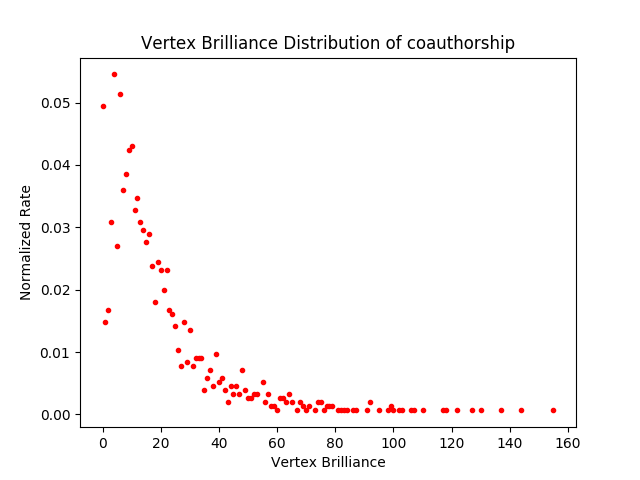
\includegraphics[width=14.5cm]{coauthorship-vertex-brilliance.png}
\subsubsection*{PA Graph}
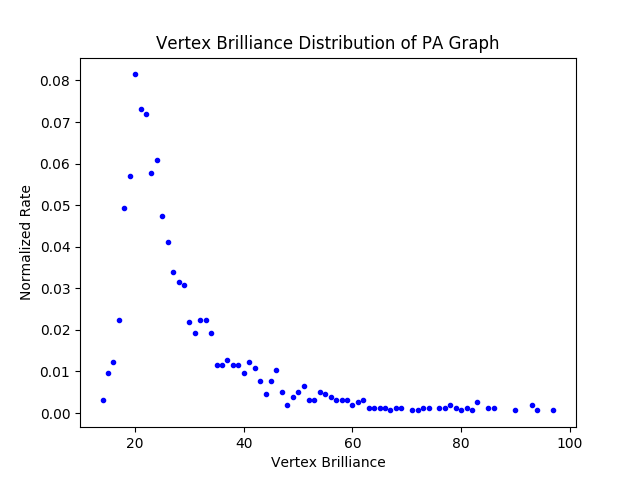
\includegraphics[width=14.5cm]{pa_graph-1559-30-brilliance.png}
\subsubsection*{Ring Group Graph}
\includegraphics[width=14.5cm]{{ring_group_graph-60-26-0.22-0.03-brilliance}.png}

\section*{Question 3}
The search time for a given start and target is the total number of queries made in reaching the target from the start (the number of intermediate vertices is not counted). The search time for a graph is the average search time over all pairs of start and target vertices. Clearly these times depend on the algorithm used for deciding when to query, when to move to a new vertex and how to decide which vertex to move to. The aim is that the search time is as small as possible.\\ \\
\noindent
Note that the array of neighbours of a vertex should not be considered ordered. If you create graphs in such a way that the neighbours are ordered, then either randomize the ordering or, when querying the array of neighbours, choose a random member of the array (from amongst those not already queried).

\begin{itemize}
    \item describe an algorithm for searching in the graphs. (I expect that you will have different algorithms for the different types of graphs.) 
    \item You should explain why you believe your strategy might be effective and implement and test it on many instances. You can choose the parameters yourself as long as you are not perverse — for example, the groups in the Ring Group Graph should not be of size 1 or n — and it is acceptable that all your testing for a particular type of graph is on instances generated with the same parameters. 
    \item As searching on graphs that are not connected can be impossible, you should choose parameters so that the graphs are very likely to be connected. 
    \item Plot search time against the number of instances that achieve that time. Comment on your plots. It is acceptable to estimate search time by looking at only a sample set of pairs of vertices. 
    \item Credit will be given for the effectiveness of the algorithm you design, and also, independently, for your explanation of the rationale behind the design.
\end{itemize}

\subsection*{Search Random Graph}
for Random Graphs, each vertex is labelled with a unique integer between 1 and n.
\subsubsection*{Algorithm}

\begin{algorithmic}
    \If {$i\geq maxval$}
        \State $i\gets 0$
    \Else
        \If {$i+k\leq maxval$}
            \State $i\gets i+k$
        \EndIf
    \EndIf
\end{algorithmic}

\subsection*{Search Ring Group Graph}
for Ring Group Graphs, each vertex is assigned a unique integer and the label of its group (see
Question 1)

\end{document}